\documentclass{article}

\usepackage{amsthm}
\usepackage{amsfonts}
\usepackage{amsmath}
\usepackage{amssymb}
\usepackage{fullpage}

\usepackage{graphicx}

\usepackage[usenames]{color}
\usepackage{hyperref}
  \hypersetup{
    colorlinks = true,
    urlcolor = blue,       % color of external links using \href
    linkcolor= blue,       % color of internal links 
    citecolor= blue,       % color of links to bibliography
    filecolor= blue,        % color of file links
    }
    
\usepackage{listings}

\definecolor{dkgreen}{rgb}{0,0.6,0}
\definecolor{gray}{rgb}{0.5,0.5,0.5}
\definecolor{mauve}{rgb}{0.58,0,0.82}

\lstset{frame=tb,
  language=haskell,
  aboveskip=3mm,
  belowskip=3mm,
  showstringspaces=false,
  columns=flexible,
  basicstyle={\small\ttfamily},
  numbers=none,
  numberstyle=\tiny\color{gray},
  keywordstyle=\color{blue},
  commentstyle=\color{dkgreen},
  stringstyle=\color{mauve},
  breaklines=true,
  breakatwhitespace=true,
  tabsize=3
}

\theoremstyle{theorem} 
   \newtheorem{theorem}{Theorem}[section]
   \newtheorem{corollary}[theorem]{Corollary}
   \newtheorem{lemma}[theorem]{Lemma}
   \newtheorem{proposition}[theorem]{Proposition}
\theoremstyle{definition}
   \newtheorem{definition}[theorem]{Definition}
   \newtheorem{example}[theorem]{Example}
\theoremstyle{remark}    
  \newtheorem{remark}[theorem]{Remark}


\title{CPSC 406}
\author{Tyler Lewis  \\ Chapman University}

\date{\today}

\begin{document}

\maketitle

\begin{abstract}
A very short introduction to typesetting in LaTeX for my courses ``Programming Languages'', ``Compiler Construction'' and ``Algorithm Analysis''.
\end{abstract}

\tableofcontents

\section{Homework}\label{intro}
\subsection{HW 1}

\begin{minipage}{0.4\textwidth}
\begin{itemize}
\item[\textbf{\emph{NFA2DFA}}] In order to convert the provided NFA to DFA I considered each possible combination of P, Q, R, and S, and considered each possible combination its own state. The included figure details every possible state the NFA/DFA may find itself in.
\end{itemize}
\end{minipage}%
%
\begin{minipage}{0.4\textwidth}
\begin{center}
    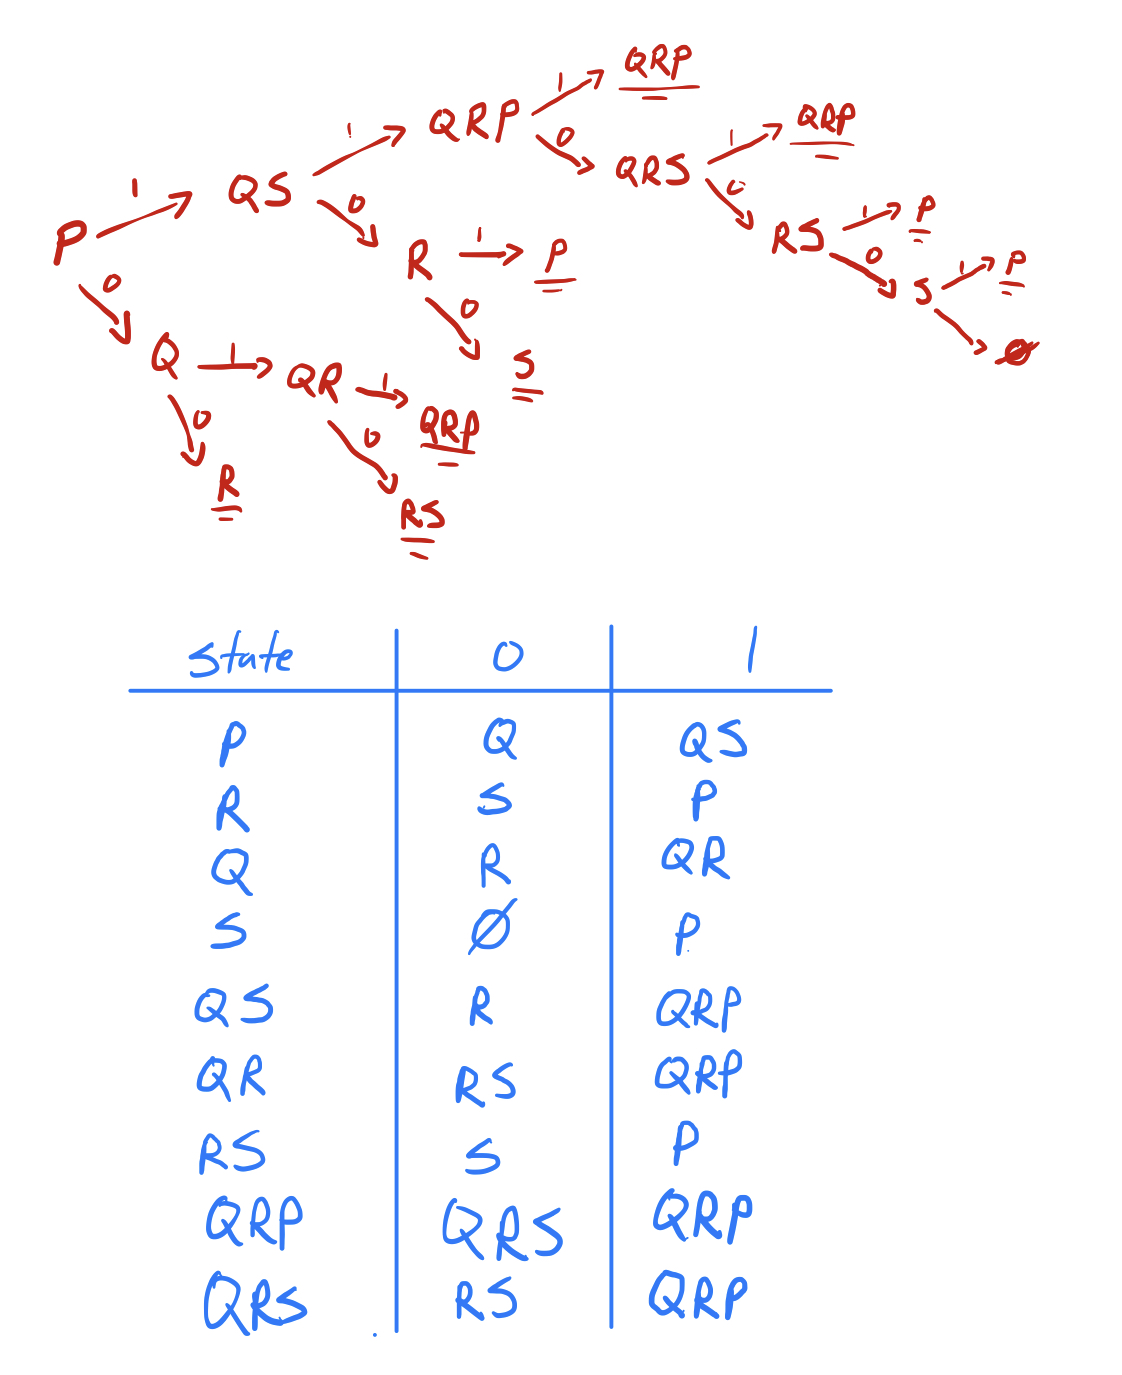
\includegraphics[width=\textwidth]{hw1.jpg}
    % \captionof{figure}{Gripper}
    \label{img:g}
\end{center}
\end{minipage}

\subsection{HW 2}

{\bf Question 1:}

    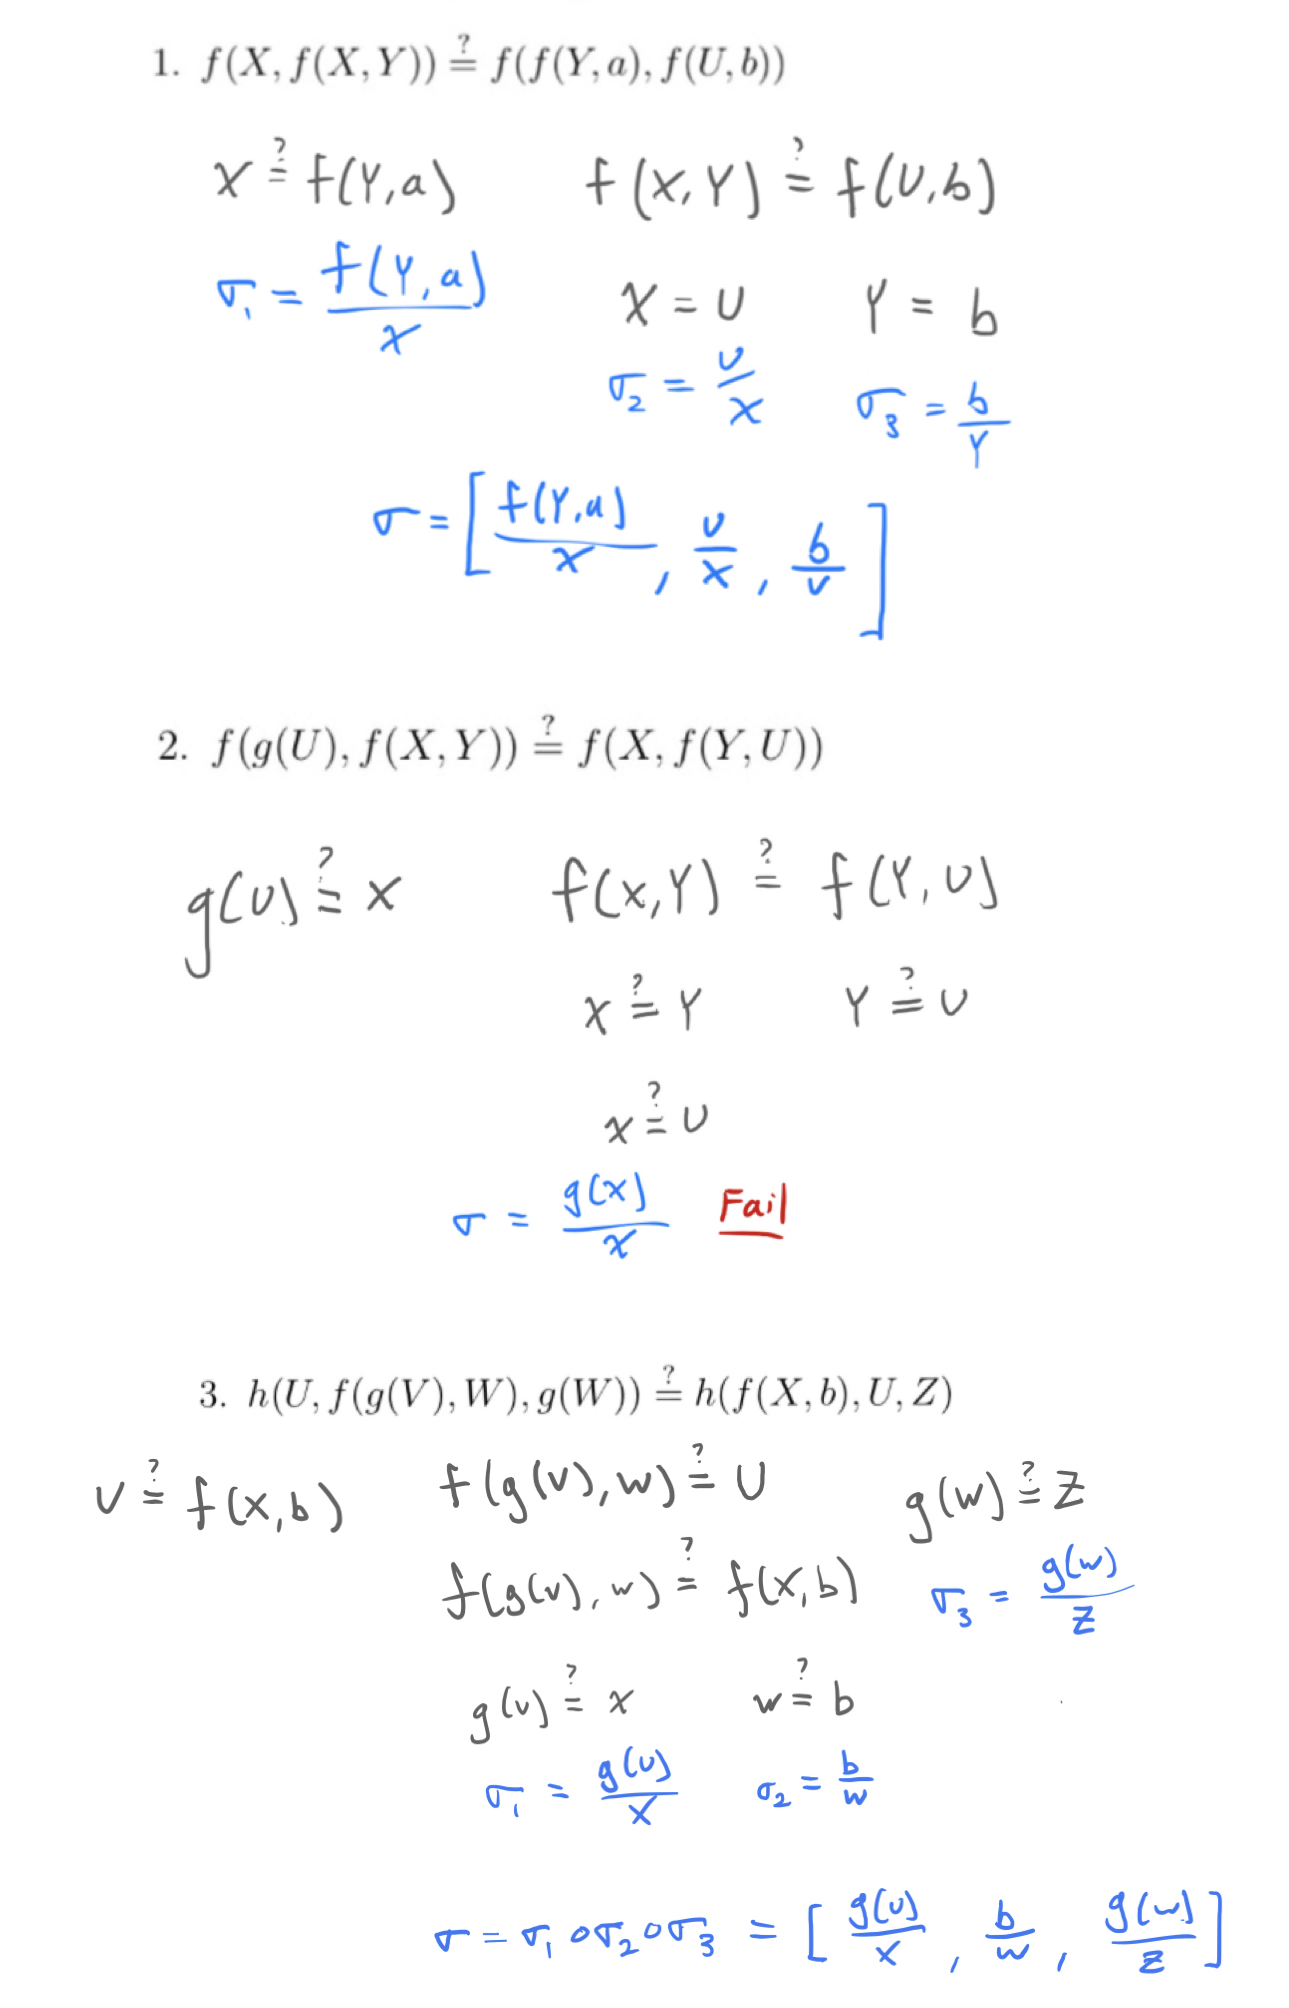
\includegraphics[width=10cm]{hw3q1.jpg}
    
% \end{center}
% \end{minipage}

{\bf Question 2:}
\texttt{
?- twoway(W,a)

?- conn(W,a), conn(a,W)

?- addr(W,a), addr(a,Z), serv(Z), addr(Z,W)
}

\subsection{HW 6}

    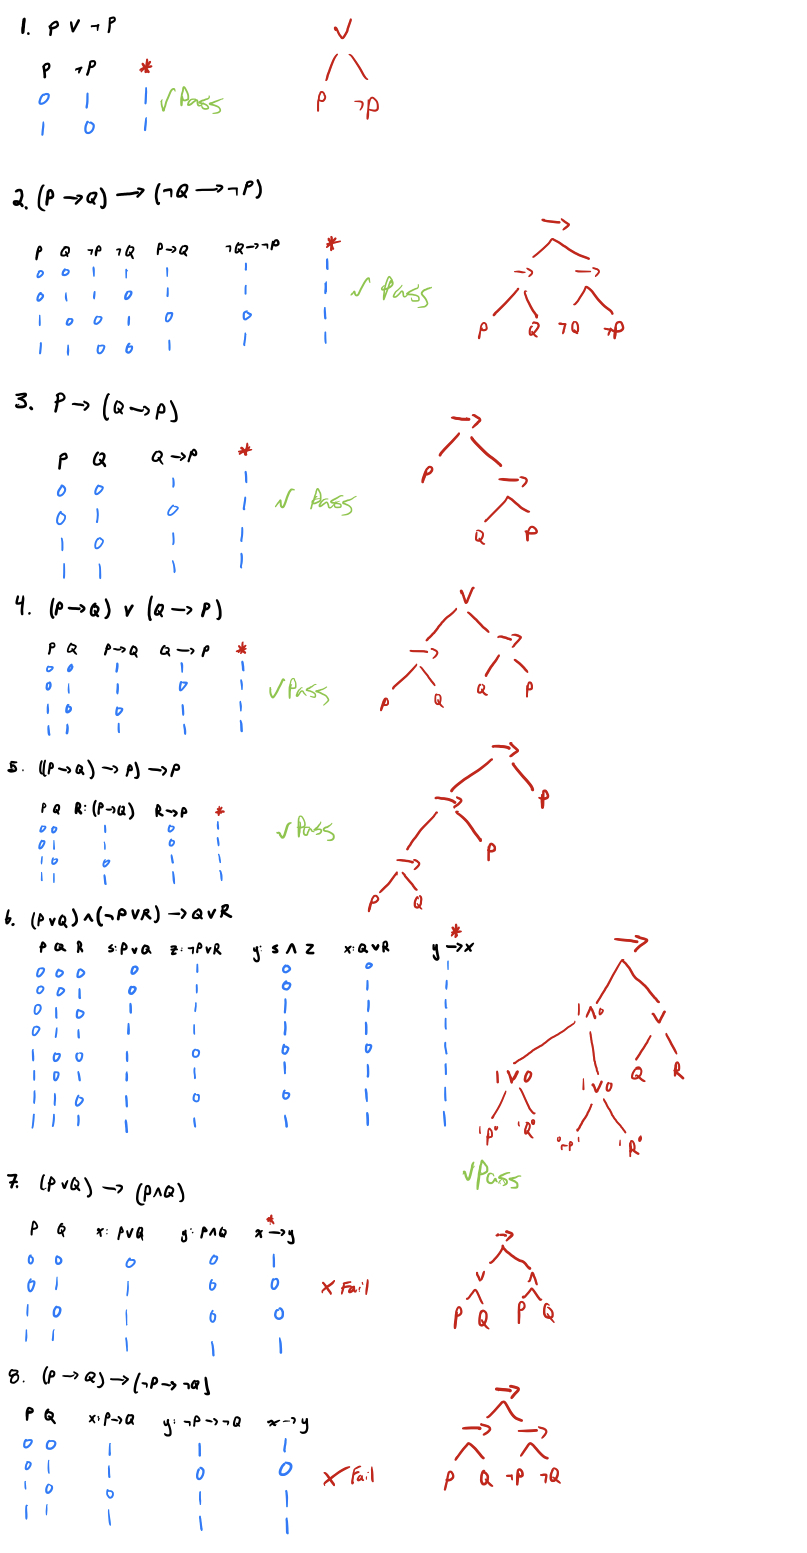
\includegraphics[width=9cm]{hw6.jpg}

\subsection{HW 9}

{\bf Exercise 1:}

\begin{itemize}
\item `success`: This is a propositional variable that is true if both statusA and statusB are ok. This variable is used to check whether the protocol was executed successfully.
\item `aliceBob`: This is a propositional variable that is true if `partnerA` is `bob`. This variable is used to check whether Alice successfully communicated with Bob.

\item `bobAlice`: This is a propositional variable that is true if `partnerB` is `alice`. This variable is used to check whether Bob successfully communicated with Alice.

\item `\&\&`: This is the logical AND operator. It is used to combine two boolean expressions and evaluate to true if both expressions are true.

\item `$\rightarrow$`: This is the implication operator. It is used to specify a condition that must be satisfied in order for an action to occur. For example, in the statement `(data.key == keyA) \&\& (data.d1 == nonceA) $\rightarrow$`, the action on the right-hand side can only occur if the conditions on the left-hand side are true.

\item `[]`: This is the "always" operator. It is used to specify a condition that must always be true in order for a property to hold. For example, the property $[] (success \rightarrow (aliceBob \land bobAlice))$ specifies that if the protocol was executed successfully, then Alice must have communicated with Bob and Bob must have communicated with Alice.

\item `[]A`: This is the "always eventually" operator. It is used to specify a condition that must eventually be true in order for a property to hold.

\end{itemize}


{\bf Exercise 2:}

The first formula, 'ltl {[] (success \&\& aliceBob -> bobAlice)} is not violated', is verified as correct, meaning that the property holds for all possible executions of the protocol. However, the second formula, 'ltl {[] (success \&\& bobAlice -> aliceBob)} is violated', is not correct, meaning that there exists at least one execution of the protocol where the property does not hold.


{\bf Exercise 3:}

The property that is violated produces an execution sequence where the specified property does not hold. Based on the trail file, the length of the execution sequence that violated the property is 84 steps. This is the total number of steps taken during the execution of the protocol before the assertion was violated.

{\bf Exercise 4:}

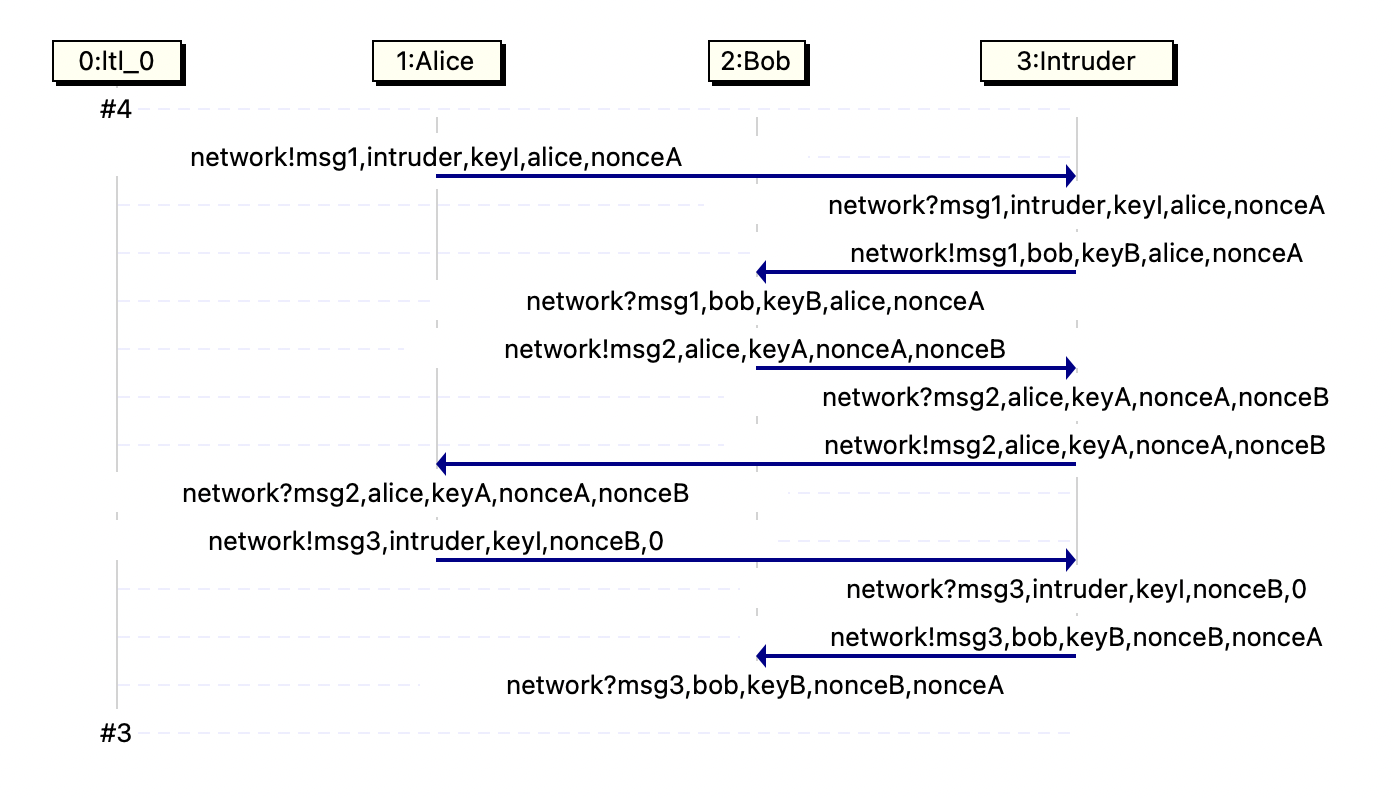
\includegraphics[width=10cm]{hw9.png}
The attack was successful because the intruder was able to intercept the messages exchanged between Alice and Bob and alter them in such a way that Alice believed she was communicating with Bob when in fact she was communicating with the intruder. Specifically, the intruder was able to send messages to Alice and sign them with Bob's key, thereby convincing Alice that she was receiving messages from Bob when in fact they were coming from the intruder.

\section{Conclusions}\label{conclusions}

In this document, to help you getting started, I gave a first succinct example of typesetting in Latex.

\begin{thebibliography}{99}
\bibitem[ALG]{Alg} \href{https://github.com/alexhkurz/algorithm-analysis-2023}{Algorithm Analysis}, Chapman University, 2023.
\end{thebibliography}

\end{document}